\begin{tcolorbox}[
        colbacktitle=gray!20,
        fonttitle=\bfseries,
        coltitle=black,
        colframe=colorrds!35!white,
        center title,
        adjusted title={Criterios de congruencia}]
    \begin{tcbitemize}[
            raster columns=4,
            raster equal height,
            raster column skip=1mm,
            size=small,
            colback=MainColor!5!white,
            colframe=MainColor!65!white,
            colbacktitle=MainColor!20!white,
            center title,
            fonttitle=\footnotesize\color{black}]
        \captionsetup[figure]{labelformat=empty}% redefines the caption setup of the figures

        \tcbitem[title={Lado Lado Lado (LLL)}]
        \begin{figure}[H]
            \centering
            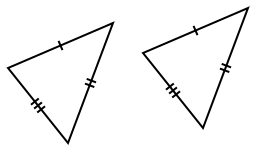
\includegraphics[width=0.9\textwidth]{../images/criterioLLL}
            \caption{Cuando los tres pares de lados correspondientes son congruentes, los triángulos son congruentes.}
            \label{fig:criterioLLL}
        \end{figure}

        \tcbitem[title={Lado Ángulo Lado (LAL)}]
        \begin{figure}[H]
            \centering
            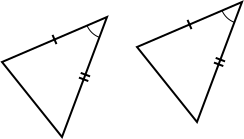
\includegraphics[width=0.9\textwidth]{../images/criterioLAL}
            \caption{Cuando dos pares de lados correspondientes y los ángulos entre ellos son congruentes, los triángulos son congruentes.}
            \label{fig:criterioLAL}
        \end{figure}

        \tcbitem[title={Ángulo Lado Ángulo (ALA)}]
        \begin{figure}[H]
            \centering
            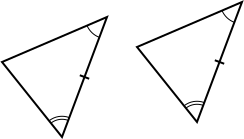
\includegraphics[width=0.9\textwidth]{../images/criterioALA}
            \caption{Cuando dos pares de ángulos correspondientes y los lados entre ellos son congruentes, los triángulos son congruentes.}
            \label{fig:criterioALA}
        \end{figure}

        \tcbitem[title={Ángulo Ángulo Lado (AAL)}]
        \begin{figure}[H]
            \centering
            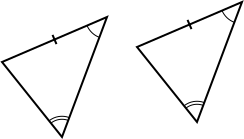
\includegraphics[width=0.9\textwidth]{../images/criterioAAL}
            \caption{Cuando dos pares de ángulos correspondientes y un par de lados correspondientes (no entre los ángulos) son congruentes, los triángulos son congruentes.}
            \label{fig:criterioAAL}
        \end{figure}
    \end{tcbitemize}
\end{tcolorbox}